\section{Human Object Tracking} \label{sec:track}
After abstracting the blob masks into feature vector representation shown in \autoref{eq:blobdenote2}, the tracking algorithm finally comes into use. To handle the one-to-many relation between blobs and actual objects, we introduce an abstract layer called object layer above the observed blob layer. The tracking algorithm maintains a list of known objects and matches an object with its optimum pair in the blob list given by the feature extractor. Every object consists of the attributes listed in \autoref{tab:objectattributes}.

 Overall speaking, the objective of the tracking layer is to:
\begin{enumerate}
  \item track the blobs by their centroid as much as possible
  \item if step 1 fails, try matching existing object with one of the central points
  \item in step 2, choose the most likely candidate for matching among all central points, considering the previous object location, motion direction as well as speed, as mentioned in \Cref{sec:featureextract}
  \item determine if two blobs actually belong to one previous object, as mentioned in \Cref{sec:detect}
  \item determine if it is an entering/ exiting event by an object's first position and last seen position, as well as modify the room occupancy count
\end{enumerate}

The above listed tracking steps are adapted from \cite{sharma2012blob} for a top-view IR image sequence, and could be further divided into two phases.

In the pairing phase, the location of an object will be updated to the paired blob location with a filter. If an object cannot find a suitable blob pair, it will not be eliminated immediately but continue propagated a few frames with the previous velocity to see if there could be a match on the forward trajectory. This is exactly the virtual track method used by \cite{virtualtrack}.

If there is at least one unmatched blob left in the blob list, the spawn phase is activated. The tracking algorithm first check if the matched blob could be a fraction of a splitted blob. If it is the case, the blob will be merged to the nearby existing object and contribute to the object location update. Finally, if the blob is unlikely to have any relation with existing objects, a new object will be spawned from the blob center.
\begin{table}
  \centering
  \begin{tabular}{|c|l|}
    \hline
    % after \\: \hline or \cline{col1-col2} \cline{col3-col4} ...
    i & unique label \\
    $\vec{x}$ & current position \\
    $\vec{\dot{x}}$ & current velocity \\
    $\vec{x_0}$ & position of first appearance \\
    $t_v$ & number of virtual track propagation \\
    \hline
  \end{tabular}
  \caption{Object attributes for tracking}\label{tab:objectattributes}
\end{table}

\subsection{Matching Step}
The objects and blobs are matched by a distance score based on nearest neighbour rule. By matching, a time disparity between the objects and blobs should be considered. Because the blobs are observed at a time step $t$, but the objects location are updated in the last time step $t-1$. By the time of matching, the objects should have already moved forward. Therefore, the blobs should be matched with the \emph{predicted position} of the objects.

A Kalman filter could be used to store the object states and predict its next state by state transition \cite{mika,virtualtrack}. Since the states in our use case only contain two components (position and velocity), and the second one is the derivative of the first one, an Alpha-Beta filter could be used to simplify the filtering process and cutdown unnecessary computational overhead.

An Alpha-Beta filter resembles the Kalman filter in its nature, combining state transition and observation for state update, but does not vary coefficients dynamically. Denote $\hat{\boldmath{x}}$ as the estimated value, $\boldmath{x}^p$ as the predicted value and $\boldmath{x}^m$ as the measured value, the system state is obtained by the following \autoref{eq:abfilter}.
\begin{equation}\label{eq:abfilter}
  \left\{
  \begin{split}
    & \hat{\boldmath{x}}_n = \boldmath{x_n}^p + \alpha\left(\boldmath{x_n}^m-\boldmath{x_n}^p\right)\\
    & \hat{\boldmath{\dot{x}}}_n = \boldmath{\dot{x}}^p_n + \frac{\beta}{T}\left(\boldmath{x_n}^m-\boldmath{x_n}^p\right)\\
    & \boldmath{x_{n+1}^p} = \hat{\boldmath{x}}_n + T \hat{\boldmath{\dot{x}}}_n\\
    & \boldmath{\dot{x}_{n+1}}^p = \boldmath{\dot{x}_{n}}
  \end{split}
  \right.
\end{equation}

In the first two lines of \autoref{eq:abfilter}, $\alpha$ and $\beta$ are two fixed coefficients that are chosen experimentally. For an camera installed at a height of 2.5m with a FOV of $60^\circ C$, we choose $\alpha=0.75,\ \beta=0.8$. \autoref{fig:trackexample1} demonstrates the smoothen effect of the filter, the estimated trajectory becomes more stable compared to the measured trajectory. More importantly, even though the filter uses fixed coefficients, the prediction usually approximate the actual measurement very well. An exception is when the human moves close to the border, because the human body is only partially detected, the centroid of that partial body stays almost still. The estimated object position will converge quickly to the actual (but wrong) measurement. This behaviour is designed intended so that the tracking could be continued.
\begin{figure}
  \centering
  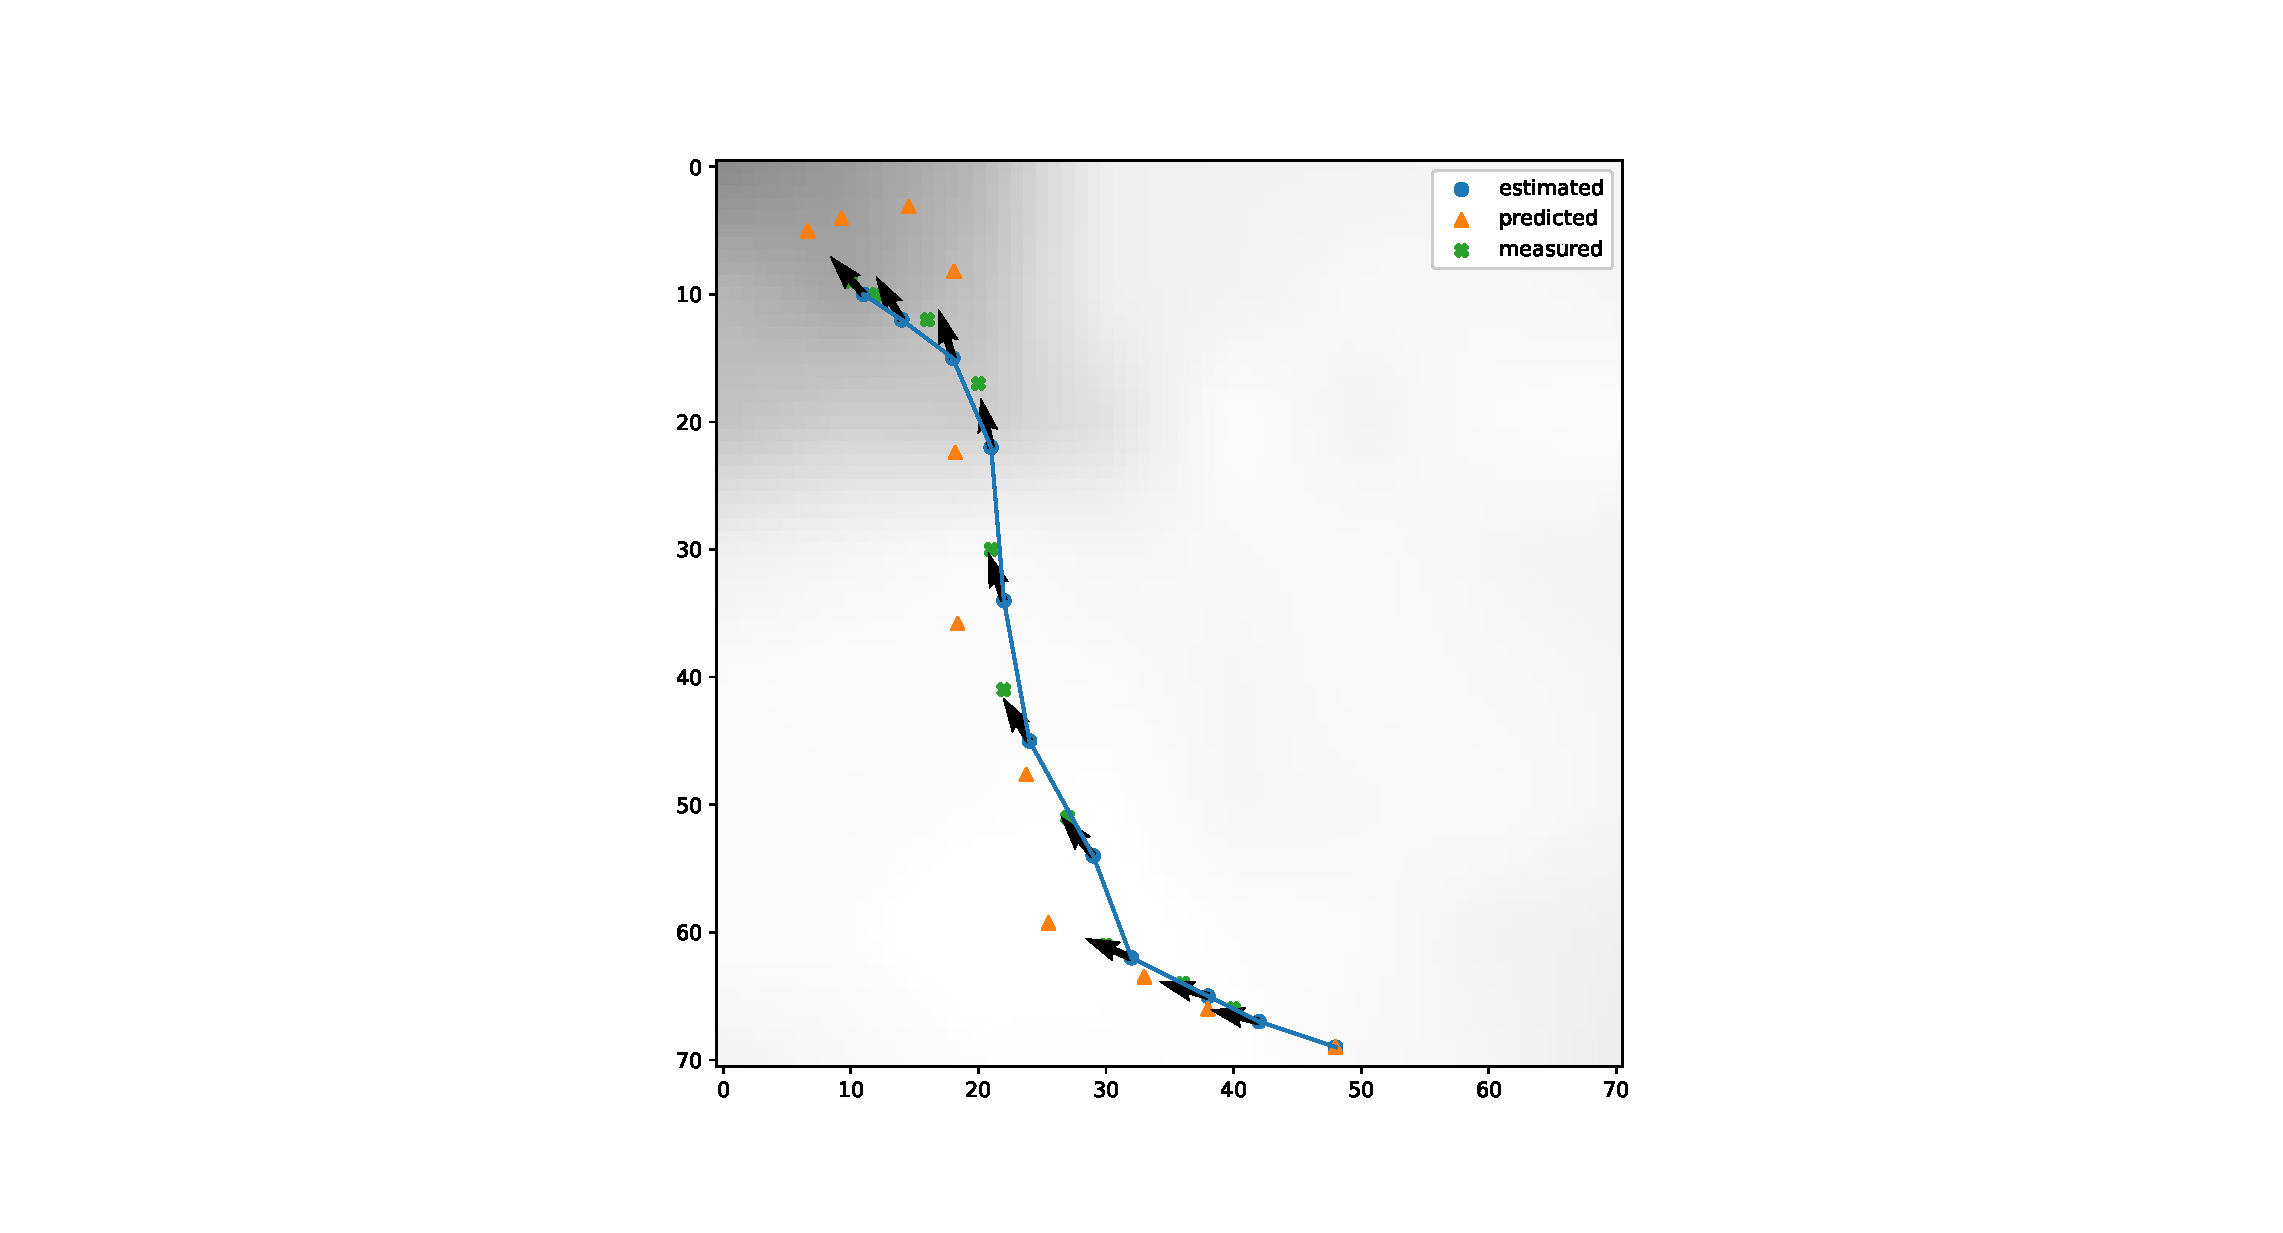
\includegraphics[width=\textwidth]{figures/trackexample1.eps}
  \caption{A track example. The blue dots show the estimated position, the arrow from the blue dot points the velocity direction of the object and the yellow triangle shows the predicted position one time step forward.}\label{fig:trackexample1}
\end{figure}

During the middle stem of the trajectory when the human is fully observed, the predicted position given by the filter significantly simplifies the tracking algorithm. The distance threshold between a blob observation and an object no longer depends on the object velocity, but merely on the prediction deviation and measurement error. Therefore, the distance threshold could be reduced to a low value, which potentially avoids false matching because of a large searching radius.

Moreover, an (relatively) accurate prediction could solve the nearest neighbour issue during central point matching mentioned in \autoref{sec:featureextract}. By central points extraction, several points on the child branch would be inevitably picked to be possible candidates, while the actual blob central must locate on the main branch. Since those points on the child branch are closer to the border and therefore closer to the last estimated object location, they will have a higher chance in pairing if we directly match the last estimated object location with the measurement. However, with one time step forward prediction, the predicted object location will locate approximately on the main branch of the central point representation, and the tracking algorithm will choose a candidate that is closer to the actual object position.

For both centroid matching and central points matching, we chose a distance threshold of 15 pixels. This value was chosen based on the camera installation height and normal walking speed.

\begin{figure}
  \centering
  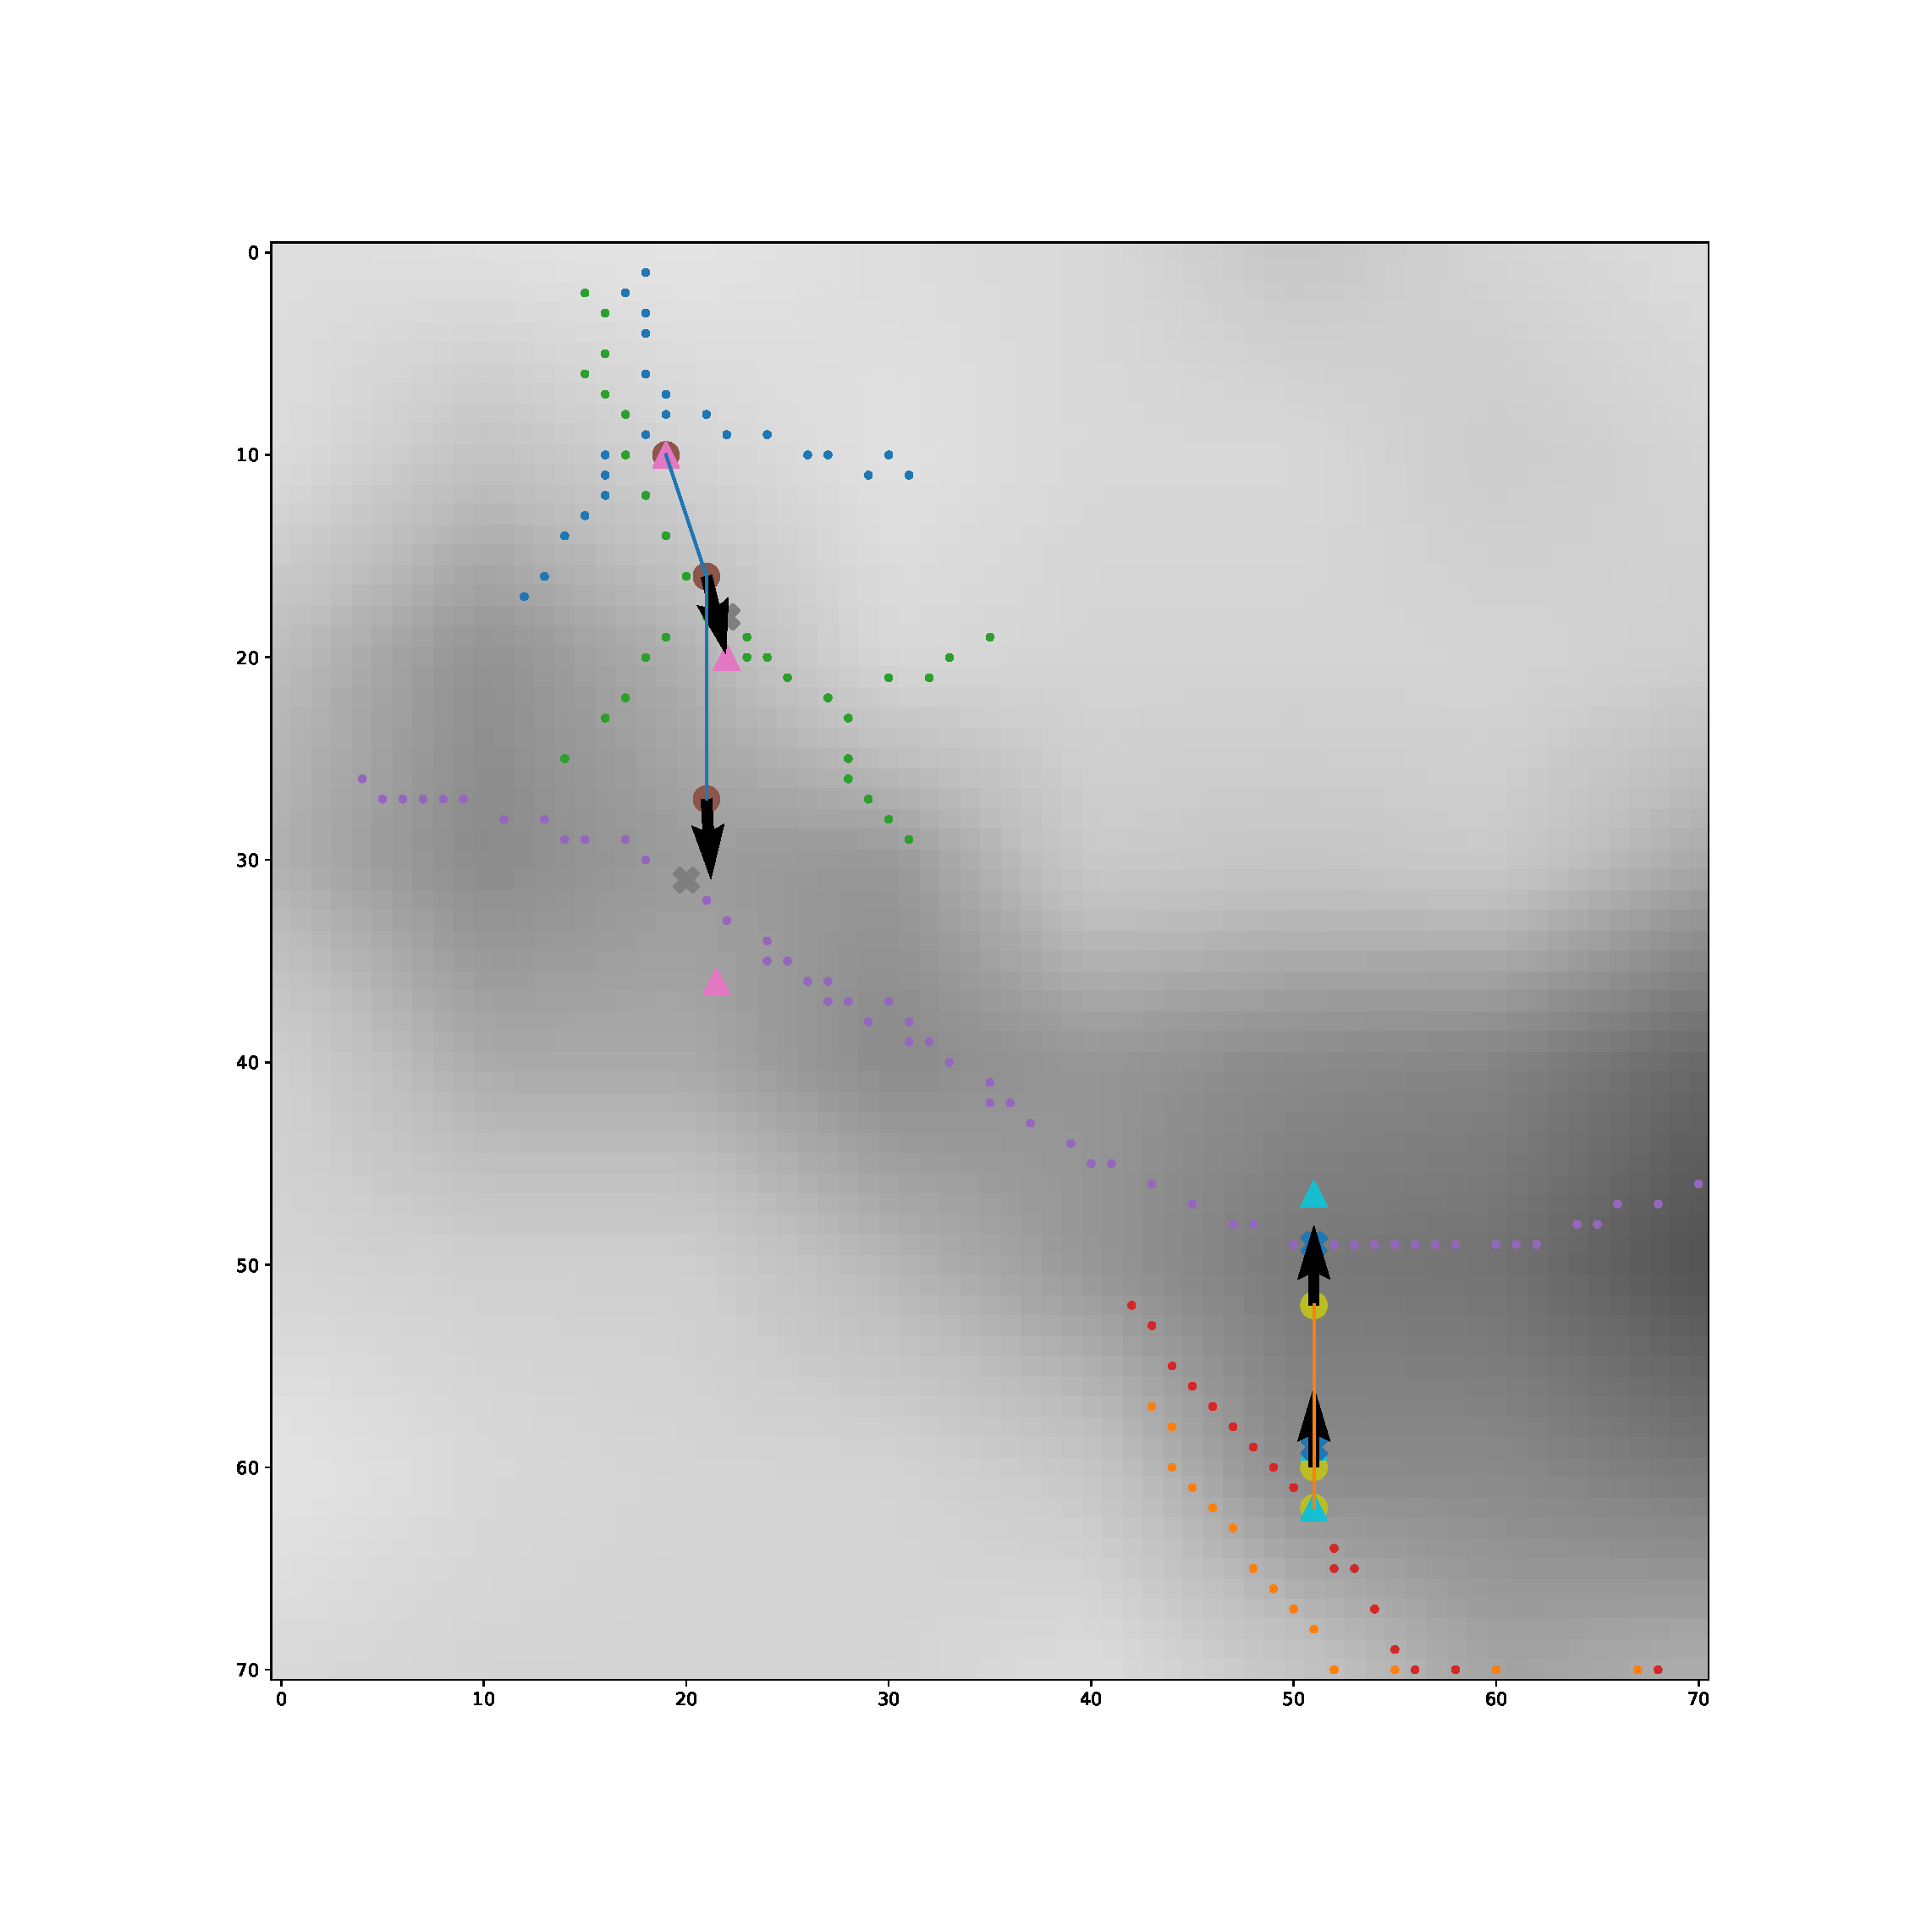
\includegraphics[width=\textwidth]{figures/trackexample2.eps}
  \caption{A track example (same sequence as \autoref{fig:blobmerge}) until two blobs merged and the central point matching is activated. The pixel dots represent the central points. The round markers are the estimated object location, triangle markers are predictions, and cross markers are measurements. The blob contour is omitted for a clear demonstration.}\label{fig:trackexample2}
\end{figure}
\begin{figure}
  \centering
  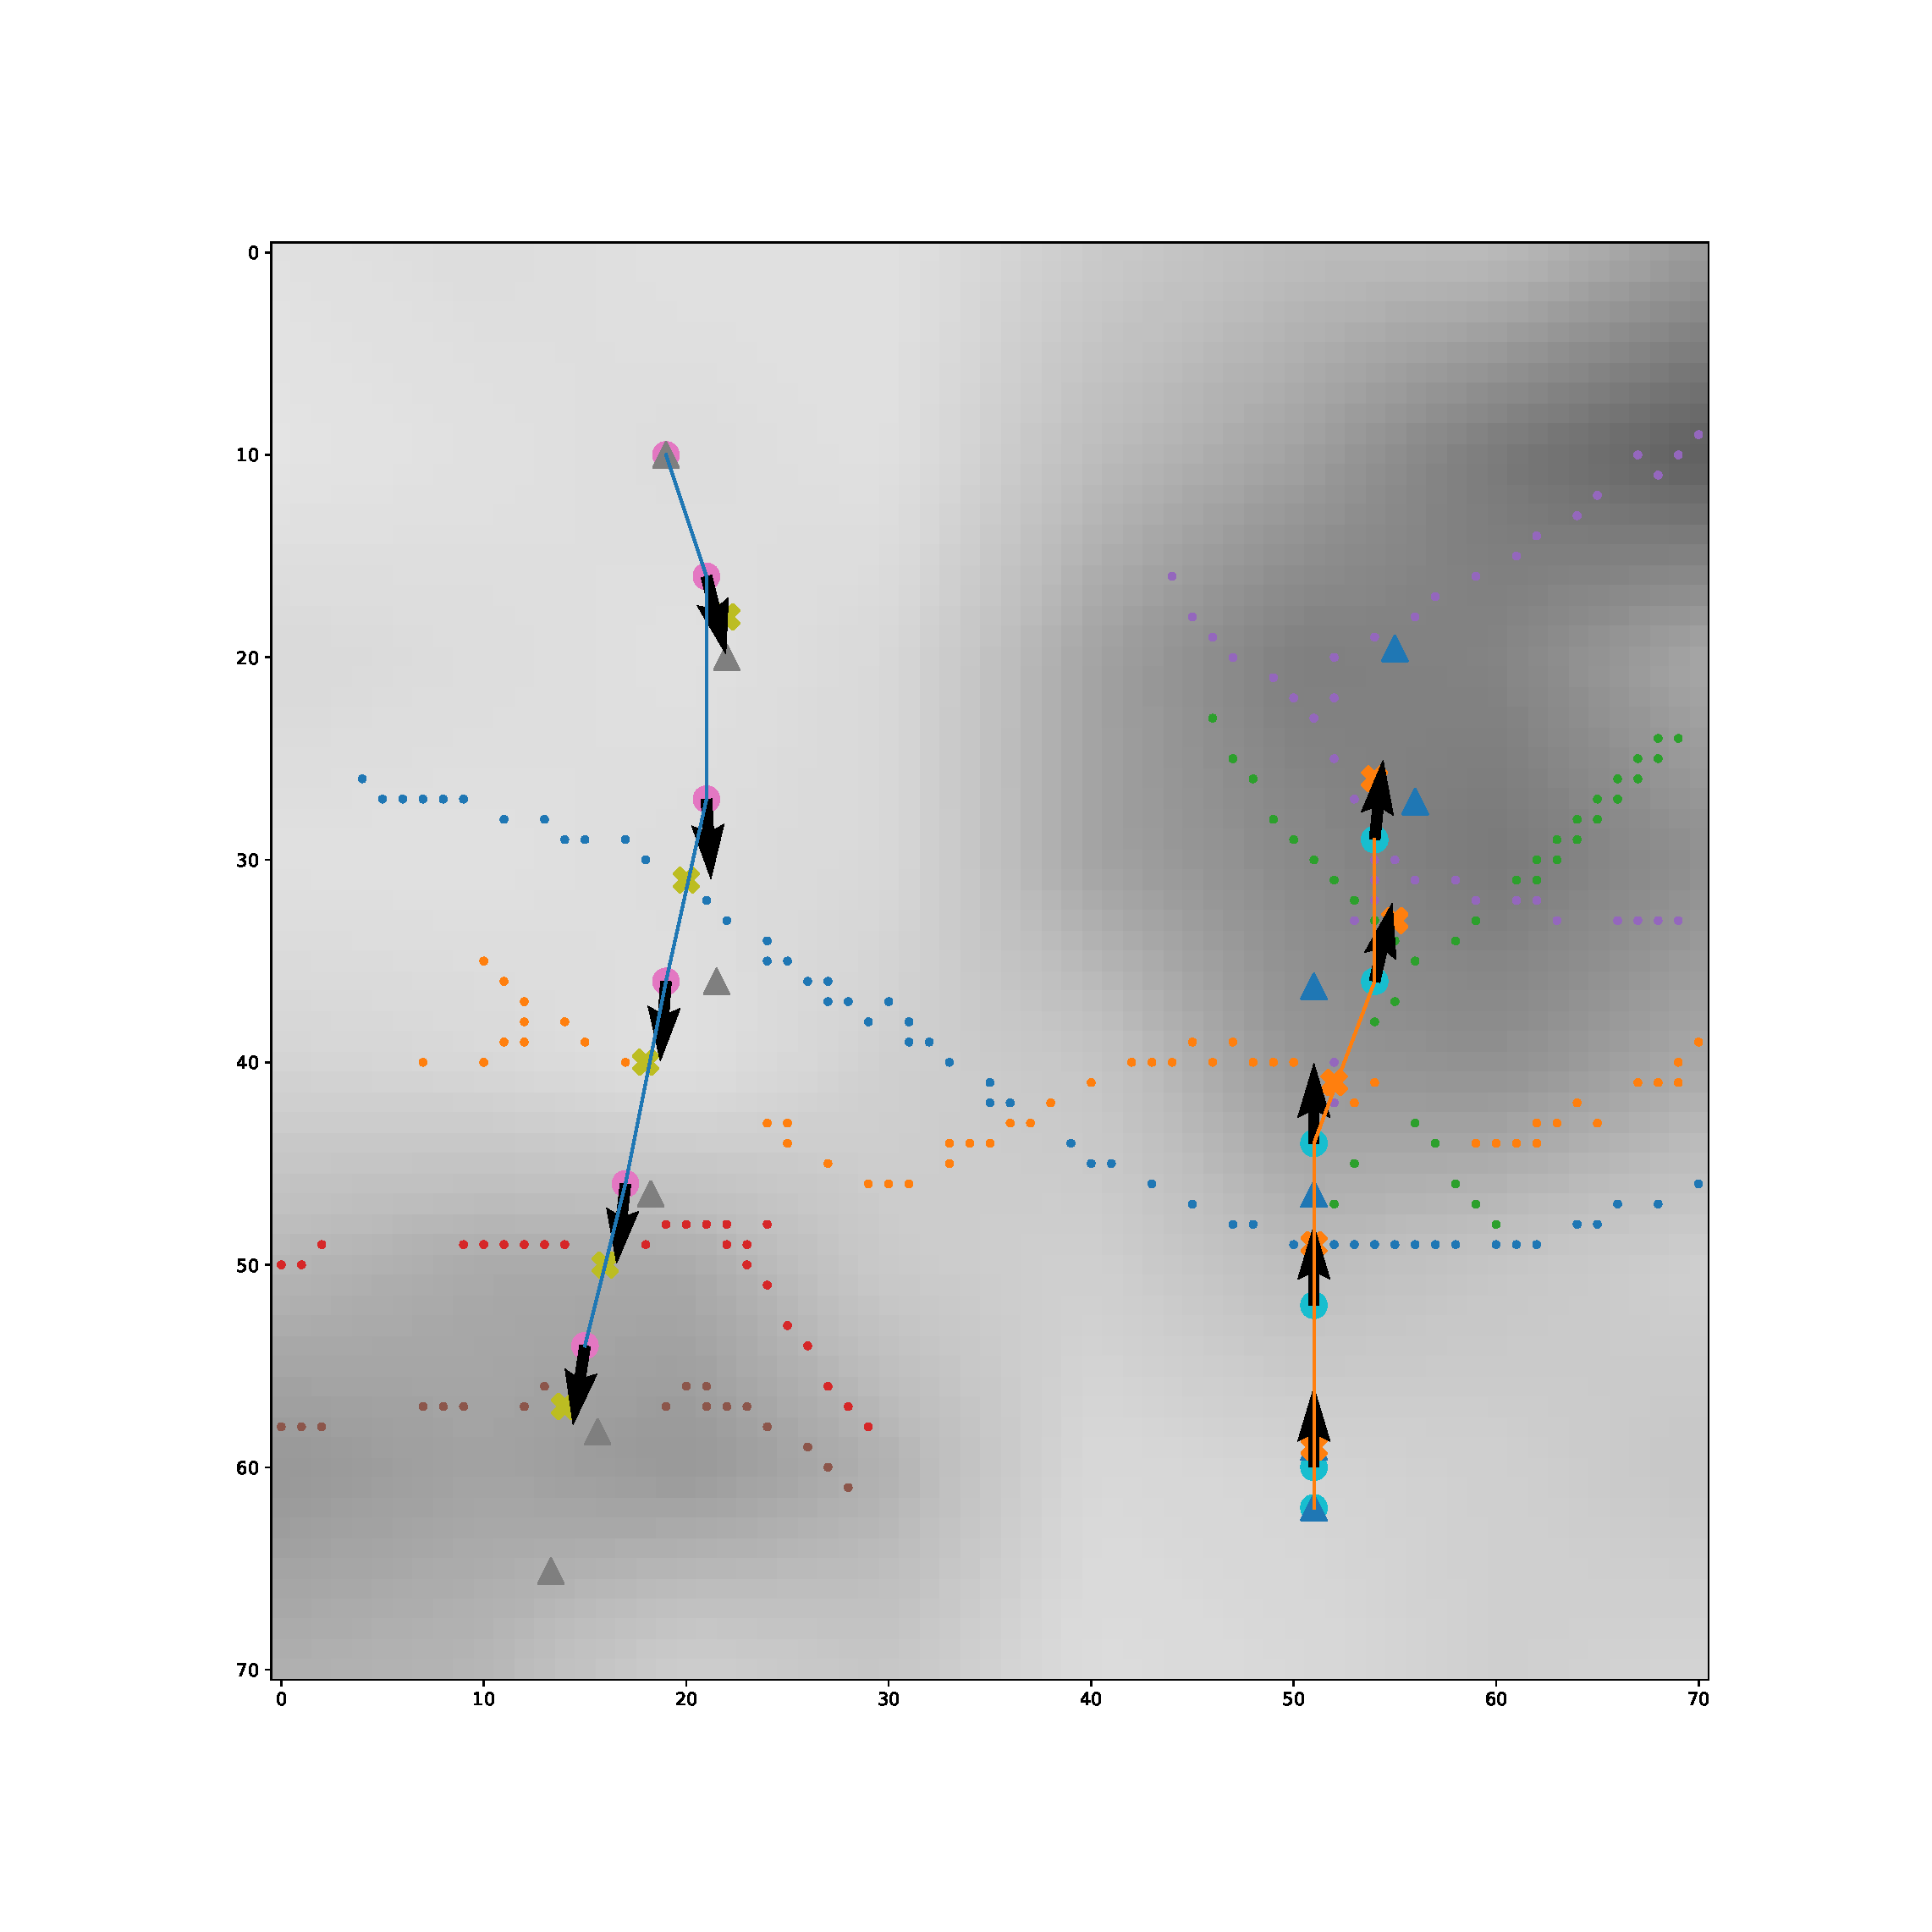
\includegraphics[width=\textwidth]{figures/trackexample2_2.eps}
  \caption{A track example (same sequence as \autoref{fig:blobmerge}, continued from \autoref{fig:trackexample2}) after the merge event. The tracking algorithm successfully handled the merging blobs and continues tracking with centroids.}\label{fig:trackexample2_2}
\end{figure}

\subsection{Virtual Track}
An event-based counting rule is applied to determine the room count value. The object activities are counted after the termination of its trajectory. A count modification of $\pm 1$ will be added to the final count if the object's first and last positions locate on different sides of the doorway middle line.

Beside the matching step based on centroid and central points, we have integrated the virtual track method proposed by \cite{virtualtrack}, though for a different purpose. We notice that sometimes in a frame sequence an object may be missing for a few frames (usually one or two). This could be traced back to the detection layer, where a human body temperature is too low, either because body temperature fluctuation or camera reading noise disturbance; or in the feature extraction layer, when the detected blob contour varies fiercely and generates a distinct central points distribution and causes a matching failure. In either case, a missing frame will immediately terminate the tracking procedure (the tracker believes the object has left the camera view) and output the relative count value by checking if the object has passed the middle line. When the missing frame happens to be the critical one bypass the middle line, the algorithm will output an incorrect relative count value: the frame sequence is separated into two individual sequences, in the first sequence an object appears on one side of the doorway, moving towards the other side and disappears before it reaches the middle line, in the second sequence another object appears from nowhere on the other side of the middle line and moves until it leaves the camera view. In both sequences, neither object has passed the middle line therefore no count is made.

To increase the robustness of our algorithm, an objected is not deleted immediately after a matching failure. Instead its location will be propagated further with previous position and velocity, which is basically a prediction with a larger time step. For the following a few frames, we try matching the predicted location with a blob. If the object is missed for just one frame, this method works very well. \autoref{fig:trackexample3} shows an example where one object is missed out for one frame because it is merged with a hotter object.
\begin{figure}
  \centering
  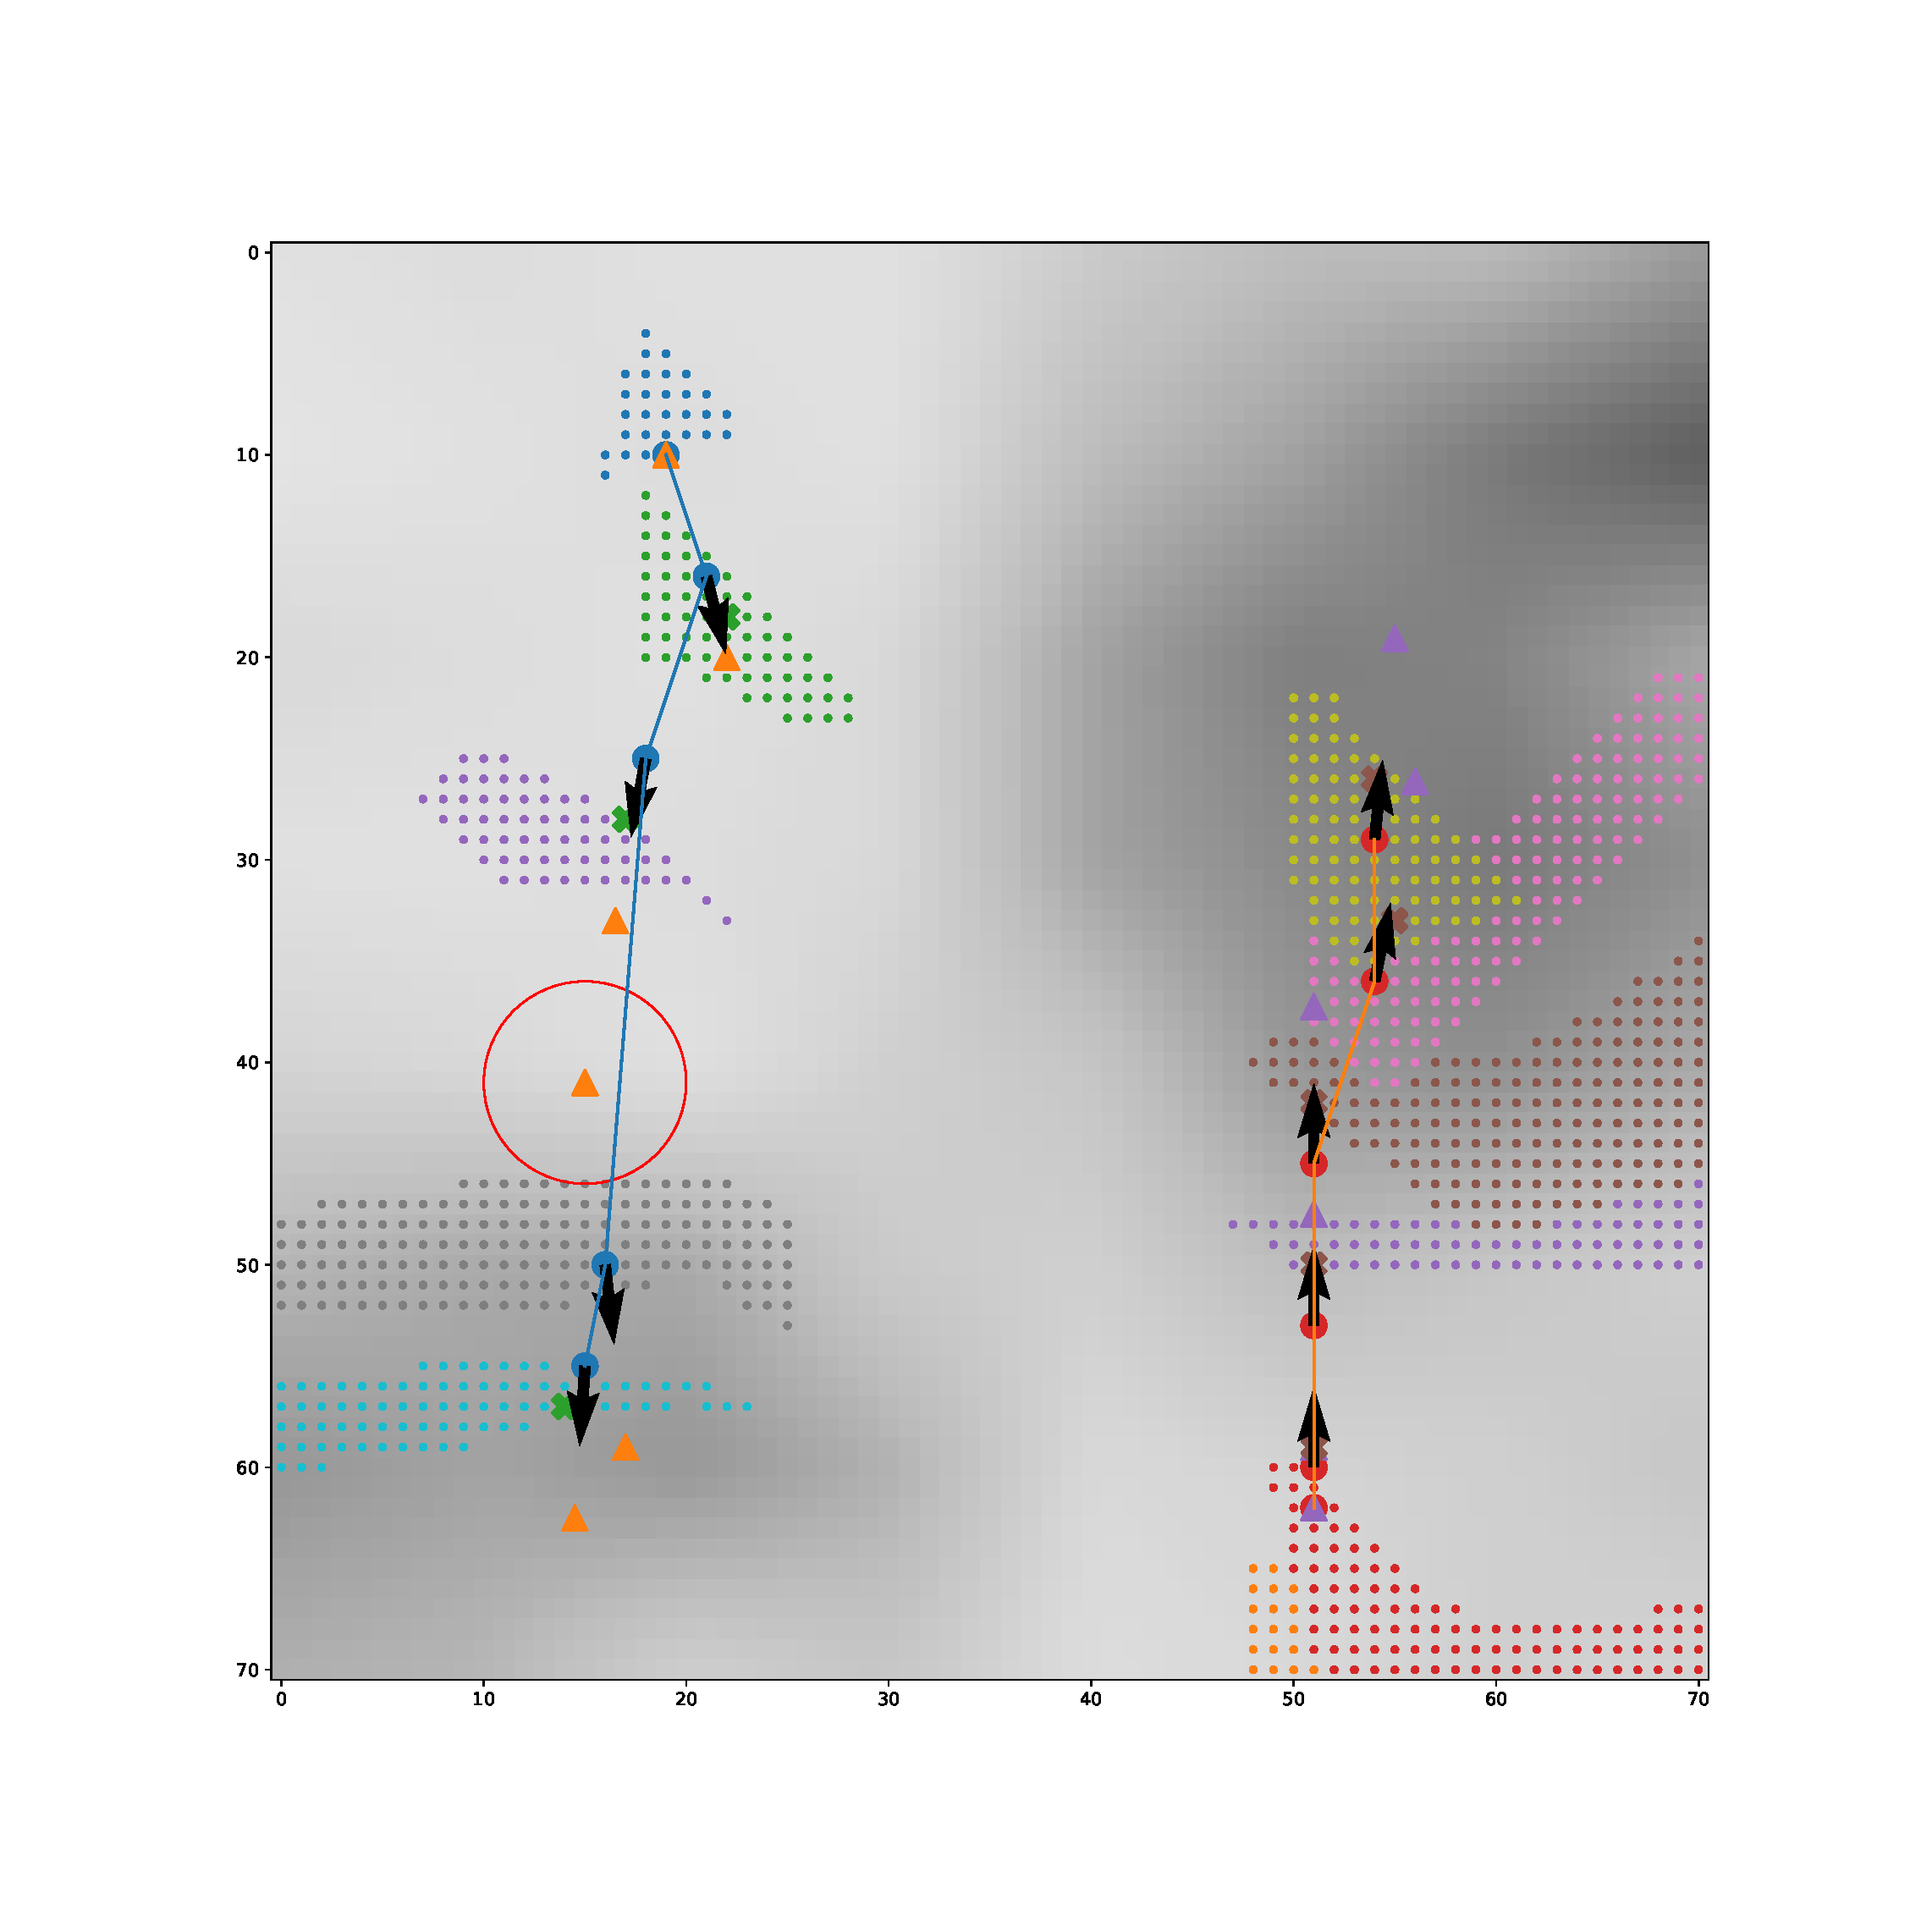
\includegraphics[width=\textwidth]{figures/trackexample3.eps}
  \caption{Virtual track propagation example (same sequence as \autoref{fig:blobmerge}), the red circle circumscribes the further transited object based on previous location and velocity. The central points are extracted with the percentage maxima distance threshold to deliberately create a detection failure. }\label{fig:trackexample3}
\end{figure}

The virtual track of an object will be created whenever an object does not find a blob to match, even when it leave the camera view. This is mainly for the ease of programm design. When an object normally leaves the camera view, its prediction of several time steps afterwards would locate out of the frame boundary, therefore it will not be incorrectly matched with a newly entered object. However, the virtual track method could only correctly predict the object location when its velocity component is non-zero. When the missing frame in a sequence happens to be the second frame, the prediction would be exactly the same as the initial position. Moreover, because the filter used for object state update, the object would only obtain a velocity component gradually. At the first few frames the object velocity has not yet converge to the actual velocity. And usually an object would only appear in the camera for about 10 frames. Therefore, the virtual track method is only meaningful in the middle section of the trajectory. This is part of the reason why we separate the entire camera view into two regions instead of three, for instance \cite{mika}, to obtain a more noise-tolerant tracking system. We choose a maxima virtual track life time to be two frames, if an object is not detected for more than two frames, it is considered a malfunction in the detection layer.

\subsection{Blob Registration}
The tracking algorithm needs to solve the splitted blob issue caused by hair isolation mentioned in \Cref{sec:detect}. A blob observation would be considered ``paired'' if it has been used to update at least one object. Otherwise it could be a new object entering the camera view. When the binary blob of an object was split into two blobs, only one of them could be matched with the corresponding object. The additional blob strongly interfere the matching procedure and could create an object that should not exist. We follow the idea of \citeauthor{sharma2012blob} \cite{sharma2012blob}, to check if a small blob could be a fraction of a previous large blob before spawning a new object from it.

The most important registration criterium is the size of the object. If a blob has splitted and part of it is used to update the object, there will be an abrupt size decay. For any unmatched blob, we check if there is a nearby object whose size just shrunk. If the size of the unmatched blob could compensate the decreased size, it is regarded as part of the object. The size of the object would be updated to the summation of two blobs' size, and the position of the object would be updated to the size-weighted average of two blobs' position.
